% \documentclass[12pt, twoside]{article}
\usepackage[letterpaper, margin=1in, headsep=0.2in]{geometry}
\setlength{\headheight}{0.6in}
%\usepackage[english]{babel}
\usepackage[utf8]{inputenc}
\usepackage{microtype}
\usepackage{amsmath}
\usepackage{amssymb}
%\usepackage{amsfonts}
\usepackage[nomessages]{fp} %\FPeval{\var-name}{2*sin(pi/6)}
\usepackage{siunitx} %units in math. eg 20\milli\meter
\usepackage{yhmath} % for arcs, overparenth command
\usepackage{tikz} %graphics
\usetikzlibrary{quotes, angles, arrows, arrows.meta}
\usepackage{graphicx} %consider setting \graphicspath{{images/}}
\usepackage{parskip} %no paragraph indent
\usepackage{enumitem}
\usepackage{multicol}
\usepackage{venndiagram}

\usepackage{fancyhdr}
\pagestyle{fancy}
\fancyhf{}
\renewcommand{\headrulewidth}{0pt} % disable the underline of the header
\raggedbottom
\hfuzz=2mm %suppresses overfull box warnings

\usepackage{hyperref}

\fancyhead[LE]{\thepage}
\fancyhead[RO]{\thepage \\ Name: \hspace{4cm} \,\\}
\fancyhead[LO]{BECA / Dr. Huson / Geometry\\*  Unit 1: Segments, length, and area\\* 19 Sept 2022}

\begin{document}

\subsubsection*{1.9 Rounding and circle area}
\begin{enumerate}
\item Write in your notebook the formulas for the area and circumference of circles and these definitions:
\begin{itemize}
  \item The radius, $r$, is the distance from the center to the edge of a circle. 
  \item The diameter, $D$, is the distance all of the way across a circle, two times the radius. $D=2r$. 
  \item The circumference, $C$, is the distance around the circle (its perimeter).
  
\end{itemize}
  \[A=\pi r^2\]
  \[C=\pi D = 2\pi r\]
  
\item Given the circle $A$ with radius $r=3$. Leave exact answers, in terms of $\pi$.
  \begin{multicols}{2}
    \begin{enumerate}
      \item Find the circumference of circle $A$. \vspace{1cm}
      \item Find the area of the circle.\vspace{2cm}
    \end{enumerate}
    \begin{flushright}
    \begin{tikzpicture}[scale=.9]
      \draw (0,0) circle [radius=3];
      \draw[fill] (0,0) circle [radius=0.05] node[below right]{$A$};
      \draw[thick, -{>[scale=1.5]}] (0,0)--(30:3);
      \node at (2,0.5){$r=3$};
      \clip (0,0) circle [radius=3];
        \draw[help lines] (-4,-4) grid (4,4);
    \end{tikzpicture}
  \end{flushright}
  \end{multicols}

\item Given the circle centered at $O$ with radius $r=3$. Leave an exact answer, in terms of $\pi$ if necessary.
  \begin{multicols}{2}
    \begin{enumerate}
      \item Find the circumference of circle $O$. %\vspace{1cm}
      \item Find the area of the circle.\vspace{2cm}
    \end{enumerate}
    %\columnbreak
    \begin{tikzpicture}[scale=.635]
      \draw[help lines] (-5,-4) grid (5,4);
      %\draw[thick, ->] (-2.2,0) -- (10.4,0) node [below right] {$x$};
      %\draw[thick, ->] (0,-2.2)--(0,10.4) node [left] {$y$};
      \draw (0,0) circle [radius=3] node[below]{$O$};
      \draw[fill] (0,0) circle [radius=0.05];
    \end{tikzpicture}
  \end{multicols}

\item Find the area $A$ and circumference $C$ of a circle with radius 4 meters (in terms of $\pi$). 

\item Find the area $A$ and circumference $C$ of a circle with radius 5 feet (in terms of $\pi$). 
  
\newpage
\item In mathematics we commonly use the special, irrational number, $\pi = 3.14159265358...$. Mark and label $\pi$ on the number line below.\par \bigskip
\begin{tikzpicture}[scale=3]
  \draw[->] (0,0)--(5.1,0);
  \foreach \x in {0, 0.1,...,5.0}
    \draw[shift={(\x,0)}] (0pt,-1pt)--(0pt,1pt);
  \foreach \x in {0, 0.5,...,5.0}
    \draw[shift={(\x,0)}] (0pt,-3pt)--(0pt,3pt)node[below=20pt]{$\x$};
\end{tikzpicture} \vspace{1cm}

\item Find the area of the shape shown below composed of a rectangle and circular cap. Leave your answer as an exact value in terms of $\pi$.
\begin{flushright}
\begin{tikzpicture}[scale=.635]
  \draw[help lines] (-2,-1) grid (8,7);
  \draw[thick, ->] (-2.2,0) -- (8.4,0) node [below right] {$x$};
  \draw[thick, ->] (0,-1.2)--(0,7.4) node [left] {$y$};
  \draw[thick] (1,1)--(7,1)--(7,3)--(1,3)--cycle;
  %\draw[thick] (3,4) arc (90:270:1);
  \draw[thick] (7,3) arc (0:180:3);
\end{tikzpicture}
\end{flushright}

\item Given the circle centered at $A$ with radius $r=2$. Leave an exact answer, in terms of $\pi$ if necessary.
  \begin{multicols}{2}
    \begin{enumerate}
      \item Find the circumference of circle $A$. %\vspace{1cm}
      \item Find the area of the circle.\vspace{2cm}
    \end{enumerate}
    %\columnbreak
    \begin{flushright}
    \begin{tikzpicture}[scale=.635]
      \draw[help lines] (-4,-4) grid (4,4);
      %\draw[thick, ->] (-2.2,0) -- (10.4,0) node [below right] {$x$};
      %\draw[thick, ->] (0,-2.2)--(0,10.4) node [left] {$y$};
      \draw (0,0) circle [radius=2] node[below]{$A$};
      \draw[fill] (0,0) circle [radius=0.05];
    \end{tikzpicture}
  \end{flushright}
  \end{multicols}

\item Find the area of the shape shown below composed of a rectangle and circular cap. Leave your answer as an exact value in terms of $\pi$.
\begin{flushright}
\begin{tikzpicture}[scale=.635]
  \draw[help lines] (-1,-1) grid (7,7);
  \draw[thick, ->] (-1.2,0) -- (7.4,0) node [below right] {$x$};
  \draw[thick, ->] (0,-1.2)--(0,7.4) node [left] {$y$};
  \draw[thick] (1,1)--(5,1)--(5,4)--(1,4)--cycle;
  %\draw[thick] (3,4) arc (90:270:1);
  \draw[thick] (5,4) arc (0:180:2);
\end{tikzpicture}
\end{flushright}

\item Mark each statement true of false.
\begin{enumerate}[itemsep=0.3cm]
  \item T \quad F \qquad 3.14 is the exact value of $\pi$
  \item T \quad F \qquad $4\pi$ is the area of a circle with radius 2 in terms of $\pi$
  \item T \quad F \qquad $C = 10\pi \approx 31.4$ is an approximation
  \item T \quad F \qquad $3\sqrt{2}$ is an exact value
  \item T \quad F \qquad $0.707\dots$ is an approximation for $\displaystyle \frac{1}{\sqrt{2}}$
\end{enumerate}

\item Find the area $A$ and circumference $C$ of a circle with radius 5 feet (in terms of $\pi$). \vspace{3cm}

\item Find the area of the shape shown below composed of a rectangle and circular cap. Leave your answer as an exact value in terms of $\pi$.
\begin{flushright}
\begin{tikzpicture}[scale=.635]
  \draw[help lines] (-1,-1) grid (7,7);
  \draw[thick, ->] (-1.2,0) -- (7.4,0) node [below right] {$x$};
  \draw[thick, ->] (0,-1.2)--(0,7.4) node [left] {$y$};
  \draw[thick] (1,1)--(5,1)--(5,4)--(1,4)--cycle;
  %\draw[thick] (3,4) arc (90:270:1);
  \draw[thick] (5,4) arc (0:180:2);
\end{tikzpicture}
\end{flushright}

\item Find the \emph{perimeter} of the shape shown below composed of a rectangle and circular cap. Leave your answer as an exact value in terms of $\pi$.
\begin{flushright}
\begin{tikzpicture}[scale=.635]
  \draw[help lines] (-1,-1) grid (7,7);
  \draw[thick, ->] (-1.2,0) -- (7.4,0) node [below right] {$x$};
  \draw[thick, ->] (0,-1.2)--(0,7.4) node [left] {$y$};
  \draw[thick] (1,1)--(5,1)--(5,4)--(1,4)--cycle;
  %\draw[thick] (3,4) arc (90:270:1);
  \draw[thick] (5,4) arc (0:180:2);
\end{tikzpicture}
\end{flushright}

\item Find the area of the shape shown below composed of a rectangle and a semi-circle.
  \begin{flushright}
  \begin{tikzpicture}[scale=.635]
    \draw[help lines] (-2,-1) grid (10,7);
    \draw[thick, ->] (-2.2,0) -- (10.4,0) node [below right] {$x$};
    \draw[thick, ->] (0,-1.2)--(0,7.4) node [left] {$y$};
    \draw[thick] (1,1)--(6,1)--(6,5)--(1,5)--cycle;
    \draw[thick] (6,1) arc (-90:90:2);
  \end{tikzpicture}
\end{flushright}

\item Find the area of the shape shown below composed of a rectangle and a semi-circle.
\begin{flushright}
\begin{tikzpicture}[scale=.635]
  \draw[help lines] (-2,-1) grid (10,7);
  \draw[thick, ->] (-2.2,0) -- (10.4,0) node [below right] {$x$};
  \draw[thick, ->] (0,-1.2)--(0,7.4) node [left] {$y$};
  \draw[thick] (1,1)--(6,1)--(6,5)--(1,5)--cycle;
  \draw[thick] (6,1) arc (-90:90:2);
\end{tikzpicture}
\end{flushright}

\item Given circle $O$ with area $A=64 \pi$ square centimeters. Find the radius, $AB$.
\begin{multicols}{2}
  \begin{tikzpicture}[scale=0.8]
    \draw (0,0) circle[radius=3];
    \draw[fill] (0,0) circle [radius=0.08];
    \draw[thick, <->]
      (0:3) node[right]{$B$}--
      (0.1,0) node[left=5pt]{$A$};
    \draw (1.5,0) node[below]{$r=?$};
  \end{tikzpicture} \par
 Start with the formula \par \smallskip
$A = \pi r^2 = 64 \pi$
\end{multicols} \vspace{1cm}


\newpage
\item One side of the $\triangle ABC$ has a length $AB=8$. The triangle's area is 44. Find the length of the altitude $h$ of the triangle to vertex $C$ and perpendicular to side $\overline{AB}$. \par
  \begin{tikzpicture}[scale=1, rotate=-40]
    \draw[thick]
      (2,0)node[below]{$A$}--
      (8,0)node[below]{$B$}--
      (5,3)node[above]{$C$} --(2,0);
    \draw[dashed] (5,0)--(5,3);
    \draw (5,0)++(0.3,0)--++(0,0.3)--+(-0.3,0);
    \node at (5,1)[right]{$h=?$};
    \node at (5,0)[below left]{$8$};
  \end{tikzpicture}

\item One side of the $\triangle ABC$ has a length $AB=12$. The triangle's area is 60. Find the length of the altitude $h$ of the triangle to vertex $C$ and perpendicular to side $\overline{AB}$.\par
\begin{tikzpicture}[scale=0.9, rotate=30]
  \draw[thick]
    (2,0)node[below]{$A$}--
    (8,0)node[below]{$B$}--
    (5,3)node[above]{$C$} --(2,0);
  \draw[dashed] (5,0)--(5,3);
  \draw (5,0)++(0.3,0)--++(0,0.3)--+(-0.3,0);
  \node at (5.2,1.5)[right]{$h=?$};
  \node at (5,-0.5)[below left]{$12$};
\end{tikzpicture}

\item Find the area of $\triangle ABC$ shown below (not actual size) with $m\angle C=90^\circ$ and the lengths of the triangle's sides as $a=3$, $b=4$, and $c=5$. 
\begin{flushright}
\begin{tikzpicture}[scale=1.4]
  \draw[thick]
  (0,0)node[left]{$A$}--
  (4,0)node[below right]{$C$}--
  (4,2.31)node[right]{$B$}--cycle;
  \draw (4,0)++(-0.3,0)--++(0,0.3)--+(0.3,0);
  \node at (2,0)[below]{$b=4$};
  \node at (4,1.2)[right]{$a=3$};
  \node at (1.8,1.4)[above]{$c=5$};
\end{tikzpicture}
\end{flushright}
\vspace{1cm}

\item Find the area of $\triangle ABC$ shown below (not actual size) with $m\angle C=90^\circ$ and the lengths of the triangle's sides as $a=50$, $b=87$, and $c=100$. \par \medskip
  \begin{tikzpicture}[scale=1.4]
    \draw[thick]
    (0,0)node[left]{$A$}--
    (4,0)node[below right]{$C$}--
    (4,2.31)node[right]{$B$}--cycle;
    \draw (4,0)++(-0.3,0)--++(0,0.3)--+(0.3,0);
    \node at (2,0)[below]{$b=87$};
    \node at (4,1.2)[right]{$a=50$};
    \node at (1.8,1.4)[above]{$c=100$};
  \end{tikzpicture}

\item The compound shape shown below is composed of a square with side length 5 cm and a triangle with base 2 cm. Find the total area of the combined shape.
  \vspace{1cm} 
  \begin{flushleft}
  \begin{tikzpicture}
    \draw[thick] (0,0)--(7,0)--(5,5)--(0,5)--cycle;
    \draw[dashed] (5,0)--(5,5);
    \node at (6, -0.5){2};
    \node at (2.5, -0.5){5};
    \node at (-0.5, 2.5){5};
  \end{tikzpicture}
  \end{flushleft} \vspace{1cm}
\item Repeat the calculation for the figure above using the trapezoid area formula. \vspace{1cm}

\item On the grid below, accurately draw and label two adjacent squares, one with a side length of 4 cm, the other with a side length of 3 cm. The grid is in centimeters.\\*[5pt]
  Find the area $A$ and perimeter $P$ of combined shape.
  \begin{flushleft}
    \begin{tikzpicture}[scale=0.2]
      \draw[help lines] (-4,-3) grid (5,3);
      %\draw[thick, ->] (-2.2,0) -- (10.4,0) node [below right] {$x$};
      %\draw[thick, ->] (0,-2.2)--(0,10.4) node [left] {$y$};
      %\draw (0,0) circle [radius=3] node[below]{$C$};
      %\draw[fill] (0,0) circle [radius=0.05];
      %\draw[thick, -] (-3,-3)--(4,-3);
    \end{tikzpicture}
  \end{flushleft}

\item On the graph, draw polygon ABCDEF with vertices A(1, 1), B(1, 4), C(3, 4), D(3, 7), E(8, 7), and F(8, 1). Find the perimeter and the area of the polygon.
\begin{flushleft}
  \begin{tikzpicture}[scale=.2]
    \draw[help lines] (0,0) grid (10,10);
    \draw[thick, ->] (0,0) -- (10.4,0) node [below right] {$x$};
    \draw[thick, ->] (0,0)--(0,10.4) node [right] {$y$};
    \foreach \x in {1,...,10}
    \draw[shift={(\x,0)}] (0pt,-3pt)--(0pt,3pt) node[below=5pt] {$\x$};
    \foreach \y in {1,...,10}
    \draw[shift={(0,\y)}] (-3pt,0pt)--(3pt,0pt) node[left=5pt] {$\y$};
  \end{tikzpicture}
  \end{flushleft}

\item Draw and label a triangle $\triangle ABC$ with base $\overline{AB}$ 8 centimeters long and altitude of 5 centimeters. (show the altitude as a dotted line, and make sure it is perpendicular to the base) 



\end{enumerate}
\end{document}